\ifx\pdfoutput\undefined
\documentclass[a4paper]{article}
\else
\documentclass[pdftex,a4paper]{book}
\usepackage{thumbpdf}
\usepackage[pdftex,bookmarks,colorlinks=true]{hyperref}

\def\pdfBorderAttrs{/Border [0 0 0] }
\fi
% ---------------------------------------------------------------------------------------------

%\usepackage{amsmath}
\usepackage{graphicx}
\usepackage{color}
\usepackage[draft]{pdfdraftcopy}
\usepackage{fancyvrb}
\usepackage{picinpar}
\usepackage{wrapfig}

% ---------------------------------------------------------------------------------------------

\DefineVerbatimEnvironment{Code}{Verbatim}
{frame=single,fontsize=\small,tabsize=4,samepage=true,numbers=left,numbersep=5pt}

\DefineVerbatimEnvironment{TightCode}{Verbatim}
{frame=single,fontsize=\tiny,tabsize=4,samepage=true,numbers=left,numbersep=5pt}

\newcommand{\freemason}{\textit{Freemason}}
\newcommand{\name}[1]{\emph{#1}}
\newcommand{\nameb}[1]{\textbf{\emph{#1}}}
\newcommand{\concept}[1]{\textit{#1}}
\newcommand{\conceptb}[1]{\textbf{\textit{#1}}}

% ---------------------------------------------------------------------------------------------

\setlength{\oddsidemargin}{0cm}
\setlength{\evensidemargin}{0cm}
\setlength{\textwidth}{16cm}
\setlength{\textheight}{23cm}

% ---------------------------------------------------------------------------------------------
\begin{document}

\pagestyle{empty}

% ---------------------------------------------------------------------------------------------

\begin{titlepage}
\draftstring{}
\watermarkgraphic{cover.pdf}
\watermark

\pdfbookmark{Cover Page}{cover}
\mbox{}
\end{titlepage}
\newpage

\watermarkgraphic{}
\mbox{}
\newpage

% ---------------------------------------------------------------------------------------------

\pdfbookmark{The \freemason\ Build System}{title}
\begin{minipage}{\textwidth}

\draftstring{}
\watermarkgraphic{../graphics/rv-frontpage-a4.pdf}
\watermark

\vspace*{2 cm}

\center{\begin{Huge} The \freemason\ Build System \par \vspace{.5 cm} Version 4.0\end{Huge}}
\par \vspace{1 cm}

\center{ \includegraphics[width=7cm]{../graphics/freemason-logo.jpg}}
\\ \vspace{2 cm}

\begin{Huge}User Guide \end{Huge}
\\ \par \vspace{0.3 cm}
\begin{normalsize}version 1.0\end{normalsize}
\par \vspace{1 cm}

%Rafi Einstein
\par \vspace{1 cm}

\today
\end{minipage}
\newpage

% ---------------------------------------------------------------------------------------------

\watermarkgraphic{}
\draftstring{}
\watermark

\begin{center}
\includegraphics[width=13cm]{governance.jpg}
\end{center}
\begin{quote}
    Then they said, "Come, let us build ourselves a city, with a tower that reaches to the heavens,
    so that we may make a name for ourselves and not be scattered over the face of the whole earth."

    -- Genesis 11:4
\end{quote}

\newpage

% ---------------------------------------------------------------------------------------------

\pdfbookmark{Table of Contents}{tableofcontents}
\tableofcontents
\newpage

% ---------------------------------------------------------------------------------------------

\pagenumbering{arabic}
\setcounter{page}{1}
\pagestyle{headings}

% ---------------------------------------------------------------------------------------------
\part{Getting Started with \freemason}

% ---------------------------------------------------------------------------------------------
\chapter{An Introduction}

\freemason\ is a build system. Its purpose is to build multi-platform software products from source code,
in a coherent and a concise way, by a single, simple command, with no user intervention.
One typical use of such facility is within a continuous integration system, which enables automatic
software build and testing to take place.
\\
While being biased towards C/C++ projects, it can be used to compile any source code that has 1-to-1 source-to-object
relations, such as Java or C\#. In addition, it can be used to perform operation that span source files and modules.
\\
In this manual, we first go over the basic features of \freemason\ by reviewing a sample project. Then we'll examine
\freemason's architecture and study its features more thoroughly.

%TBD: build definition files as source code

% ---------------------------------------------------------------------------------------------
\chapter{Getting Started}

Let's take a look at a simple project, \emph{Sample1}, containing a program and a library (Figures \ref{sample1:project.1} and \ref{sample1:sources}).

\begin{figure}[h]
\caption{\label{sample1:project.1}Sample1 project}
\begin{center}\fbox{\includegraphics[height=5cm, width=7cm, keepaspectratio]{sample1/test1-1.pdf}}\end{center}
\end{figure}

\begin{figure}[h]
\caption{Sample1 project sources}
\label{sample1:sources}

\begin{center}
\begin{tabular}{cc}

\\

\begin{tabular}{c}

\verb"test1/test1.cpp"

\\

\begin{minipage}{2in}
\begin{Code}
#include "lib1/lib1.h"

#include <stdio.h>

int main()
{
    printf("%s\n", foo());
    return 0;
}
\end{Code}
\end{minipage}
\end{tabular}

&

\begin{tabular}{c}

\verb"lib1/lib1.cpp"

\\

\begin{minipage}{2in}
\begin{Code}
const char *foo()
{
    return "Hello, World!";
}
\end{Code}
\end{minipage}

\\

\\

\verb"lib1/lib1.h"

\\

\begin{minipage}{2in}
\begin{Code}
const char *foo();
\end{Code}
\end{minipage}

\end{tabular}

\end{tabular}
\end{center}

\end{figure}

\newpage
% ---------------------------------------------------------------------------------------------
\section{Makefiles}
The first thing we will like to do is to build the code in \nameb{test1} and \nameb{lib1}. We would like to build the source files in
\nameb{lib1} into a library, and the source files in \nameb{test1} into an executable file.
\freemason\ uses the term \conceptb{module} to refer to a set of source files (like \nameb{test1} and \nameb{lib1}) that eventually
can be compiled into binary form (that is, a library of some sort or an executable, which we call \conceptb{products}).
\par
For \freemason\ to build a module it needs some instructions. Those instructions are written in a language that has no name,
but it is known to its acquaintances as the language of a bloke called \name{GNU make}. This file is called, not surprisingly,
\concept{makefile}. The makefiles are placed along with the source files (Figure \ref{sample1:project.2}).
\par
Let's examine the makefile of \nameb{test1} (Figure \ref{sample1.1:makefiles}). We first define a variable called \verb"SRC_ROOT" (line 1)
that serves as an anchor to the root of our source code. Since \nameb{test1} resides under \nameb{sample1}, we go two levels up the directory
structure to meet the root.
\par
The next line introduces \freemason. We will assume here that the \freemason\ definitions files (also
called \concept{Framework}) are in \verb"z:/freemason". However, in the most common (and most recommended) configuration,
the \concept{Freemason Framework} is a of the source view. More on that later. Thus, \freemason\ is introduced by including the file
\verb"main" from the \concept{Freemason Framework}. Once it is done, the variable \verb"MK" can be used to reference \freemason\ resources.
\par
After we shook hands and got off the coats, it's time to introduce ourselves to \freemason. By defining variable \verb"MODULE_NAME" (line 4),
an arbitrary text string we set the name of the module. The name of the module should be unique in the sense
that no two modules that are used in the same context should have the same name.
\freemason\ also uses the module name to name the module's product file (the file that is created by the build process).
\par
Now, before we can haggle over the price, we should establish what we are\footnote{According to George Bernard Shaw.}. The variable \verb"PRODUCT" (line 5) does just that: it tells \freemason\ what will become out of the module once it is compiled.
Among the possible values are \verb"prog" (an .exe file or the like), \verb"lib" (.lib or .a file), and \verb"so" (.dll or .so file).
\par
In lines 10 and 27 we introduce the rest of the \concept{Framework} code: the definitions and the rules. Both are concepts
rooted in \name{GNU make} terminology. Since the implementation of the \concept{Framework} is out of our scope, we will not discuss
them here. What we need to know for now is that definition should appear before the rules, and that some variables (the ones we just
discussed) should appear before \freemason\ definitions are included.
\par
The definitions in lines 14-23 provide information related to preprocessor definitions (\verb"CC_PP_DEFS.common"), include files directories
(\verb"CC_INCLUDE_DIRS.common"), and C/C++ source files to be compiled \\(\verb"CC_SRC_FILES.common"). There are some things to notice here.
\begin{enumerate}
	\item The \verb"CC" prefix. This implies that we supply information for a C/C++ compiler abstraction, rather than to a specific compiler.
		Therefore, we see no place where proprietary compiler option can be specified. This might look strange in first sight, but bear in mind
		that we're dealing with a cross-platform, cross-compiler, cross-my-heart environment. We'll discuss ways of customizing compiler operation
        in chapters to come.
	\item The \verb".common" suffix. That's to say "for all platforms".
	\item The header files of the module. One should not specify header files in \verb"CC_SRC_FILES". \freemason\ automatically keeps
		track of header files that are used by source files.
	\item The include file directory specified for \nameb{test1}. The directory \texttt".." needed in order to allow \texttt"test1.cpp" to
		use the header file \verb"lib1/lib1.h". Using module's name as part of the header file name is considered a good practice.
\end{enumerate}
\par
The makefile of \nameb{lib1} is very similar. One noticeable difference is the \verb"PRODUCT", defined to be \verb"lib".

\begin{figure}[htbp]

\caption{\label{sample1.1:makefiles}sample1 makefiles}

\begin{center}
\begin{tabular}{ccc}

\begin{minipage}[t]{5.5cm}
\center{test1/makefile}
\begin{Code}
SRC_ROOT=../..
include z:/freemason/4/main

MODULE_NAME=test1

PRODUCT=prog

#-----------------------------

include $(MK)/defs

#-----------------------------

define CC_PP_DEFS.common
endef

define CC_INCLUDE_DIRS.common
	..
endef

define CC_SRC_FILES.common
	test1.cpp
endef

#-----------------------------

include $(MK)/rules
\end{Code}
\end{minipage}

&&

\begin{minipage}[t]{5.5cm}
\center{lib1/makefile}
\begin{Code}
SRC_ROOT=../..
include z:/freemason/4/main

MODULE_NAME=lib1

PRODUCT=lib

#----------------------------

include $(MK)/defs

#----------------------------

define CC_PP_DEFS.common
endef

define CC_INCLUDE_DIRS.common
endef

define CC_SRC_FILES.common
	lib1.cpp
endef

#----------------------------

include $(MK)/rules
\end{Code}
\end{minipage}

\end{tabular}
\end{center}

\end{figure}

\begin{figure}[htbp]
\caption{\label{sample1:project.2}Sample1 project with makefiles}
\begin{center}\fbox{\includegraphics[width=10cm, keepaspectratio]{sample1/test1-2.pdf}}\end{center}
\end{figure}

\newpage

% ---------------------------------------------------------------------------------------------
\section{Compilation}

After we're done with writing makefiles, we can turn to compilation.
\freemason\ services are provided through a single command (also called "driver"): \textbf{mk}.
\par
There are two things \freemason\ has to know before it can build a C/C++ project:
\begin{enumerate}
	\item What is the platform for which we want to build (\verb"PLATFORM" variable),
	\item Whether we're interested in a debug build (\verb"DEBUG=1") or an optimized one (\verb"OPT=1").
\end{enumerate}
\par
For the time being, we'll perform a debug build for a platform called \verb"win32", that targets x86 machines running
Windows, and uses a C++ compiler from Microsoft.
\\
\par
And so, from the \verb"sample1/lib1" directory, we issue the command \fbox{\texttt{mk PLATFORM=win32 DEBUG=1}}.
\\
\freemason\ responds with:

\begin{figure}[h]
\caption{\label{sample1:lib1:output}sample1/lib1 win32 compilation}
\begin{Code}
Build of lib1 ...

Compiling lib1.cpp ...
Creating library bin/win32-debug/lib1.lib ...
Done.
\end{Code}
\end{figure}

Looks like everything is in order here.
\\
\\
Now, from the \verb"sample1/test1" directory, we issue the command \fbox{\texttt{mk PLATFORM=win32 DEBUG=1}}.

\begin{figure}[h]
\caption{\label{sample1:test1:output.1}sample1/test1 win32 compilation (with errors)}
\begin{Code}
Build of test1 ...

Compiling test1.cpp ...
Creating program bin/win32-debug/test1.exe ...
make: *** [bin/win32-debug/test1.exe] Error 96
\end{Code}
\end{figure}

Errors. Damn software. Cannot even compile a 5-line project. And it doesn't print a proper error message! Hang the DJ!
Hey, wait a minute. There's a \verb"make.log" file (Figure \ref{sample1:test1:make.log.1}). Maybe we can find something here.
\begin{figure}[h]
\caption{\label{sample1:test1:make.log.1}sample1/test1 win32 compilation errors (make.log)}
\begin{Code}
-------------------------------------------------------------------------------
Fri Jun 13 06:66:00 JDT 2007
Build of test1 ...
-------------------------------------------------------------------------------
Compiling test1.cpp ...
test1.cpp
test1.obj : error LNK2001: unresolved external symbol
                           "char * __cdecl foo(void)" (?foo@@YAPADXZ)
bin/win32-debug/test1.exe : fatal error LNK1120: 1 unresolved externals
\end{Code}
\end{figure}

\par
As it appears, we've got ourselves an undefined symbol. Obviously, it is the function \verb"foo()", defined in \nameb{lib1}.
Since we didn't tell \nameb{test1} anything about the latter, it doesn't add the library to its link command, leaving the
symbol \verb"foo" undefined.

We have to find a way of telling \nameb{test1} about \nameb{lib1}. This is done in two stages.
First, we establish a definitions file (\verb"defs.mk", Figure \ref{sample1.1:lib1:defs.mk}) that describes
the interface of \nameb{lib1} towards other modules.
\par
Line 1 defines the module's name (corresponds to the one in \verb"makefile"). Line 2 defines the module location, relative to the
root of the project, as defined by the \verb"SRC_ROOT" in the makefiles. \freemason\ defines a variable, \verb"VROOT"
(\concept{view root}), to point to that location. It implies that all projects in a given context should have the
same root. Line 6 defines the module product type, which corresponds to the \verb"PRODUCT" in \verb"makefile".
Last but not least, Lines 4 and 8 introduce \freemason\ framework resources related to module definitions.
One may ask, where the variables \verb"MK" and \verb"VROOT" get their values from. The answer comes from the fact
that \verb"defs.mk" aren't invoked directly as main makefiles, but rather included by the \freemason\ framework
once those variables have been defined.

\begin{figure}[h]
\caption{\label{sample1.1:lib1:defs.mk}sample1/lib1/defs.mk}
\begin{Code}
MODULE=lib1
MODULE_DIR=$(VROOT)/sample1/lib1

include $(MK)/module/start

MODULE_PRODUCT=lib

include $(MK)/module/end
\end{Code}
\end{figure}

Then, we specify the modules on which \nameb{test1} depends, with \verb"depends.mk" file (Figure \ref{sample1:test1:depends.mk}). Note
that in order for a module to be a dependency of another, it has to own a \verb"defs.mk" file. The dependencies file defines the variable \verb"MODULE_DEPENDS.common", which is a sequence of expressions of the form \verb"(module-name,number-path)", similar to those that appear in the corresponding \verb"defs.mk" files.

\begin{figure}[h]
\caption{\label{sample1:test1:depends.mk}sample1/test1/depends.mk}
\begin{Code}
define MODULE_DEPENDS.common
	(lib1,$(VROOT)/sample1/lib1)
endef
\end{Code}
\end{figure}

After establishing the \verb"defs.mk" and \verb"depends.mk" files, we'll try to recompile \nameb{test1}.

\begin{figure}[h]
\caption{\label{sample1:test1:output.2}sample1/test1 win32 compilation}
\begin{Code}
Build of test1 ...

Creating program bin/win32-debug/test1.exe ...
Done.
\end{Code}
\end{figure}
This time, with more luck.

\newpage
Let's take a look at the \nameb{sample1} project directories after the build (Figure \ref{sample1:project.3}).

\begin{figure}[h]
\caption{\label{sample1:project.3}Sample1 project after win32 compilation}
\begin{center}\fbox{\includegraphics[width=\textwidth, keepaspectratio]{sample1/test1-3.pdf}}\end{center}
\end{figure}

A few notes:
\begin{enumerate}
    \item Modules: A term \concept{module} is central to \freemason. It is the basic build unit. We've already seen examples for modules (\nameb{test1} and \nameb{lib1}). For those that seek a formal definition, a module is any location that owns either \verb"makefile" or \verb"defs.mk" files, or both.

    \item Dependant modules: modules that are used by other modules called \concept{dependent modules}. The module dependency relation induces
        a /concept{Module dependency graph}. In this example, \nameb{lib1} is a dependent module of \nameb{test1}.

    \item Deep build: If we examine the build process we just performed, we notice that we executed two build commands, one for each module. However, since the modules are dependant, it's logical to expect to build both modules with one command. This can be accomplished by adding \verb"DEEP=1" to the command with which we built module \nameb{test1}. In \freemason\ terms, it's called \concept{Deep Build}, in which a module and all its dependant modules are built.

    \item \verb"bin" directory: \freemason\ stores binary files it creates (object files, libraries, executables, etc.) under \verb"bin" directory,
        followed by a directory that named after the \concept{build variant}, that is, platform and debug/optimization selection. In this example,
        we compiled for \verb"win32" platform with debug, so the binary files directory is \verb"bin/win32-debug".

    \item \verb".d" files: \freemason's automatically detects which header files are included by each C/C++ source file it compiles. It then appends \verb".d" to the name of the source file and stores the results in the binary directory.
\end{enumerate}

\newpage

% ---------------------------------------------------------------------------------------------
\section{Yet Another Platform}

Once we got hold of building using \freemason, we can go on and build for another platform, VxWorks.
\\
From \verb"sample1/test1", we issue the command \fbox{\texttt{mk PLATFORM=vxworks OPT=1 DEEP=1}}.
\\
We requested \freemason\ to build an optimized version of \nameb{test1} and \nameb{lib1} for VxWorks.
Actually, this is a bit misleading, since VxWorks compilations are compiler-dependant and architecture-dependant,
therefore there cannot be a generic "vxworks" platform. Thus we assume that our \freemason\ framework contains
a proper definition of such architecture, and that is uses a Diab compiler.

\begin{figure}[h]
\caption{\label{sample1:output.1}sample1 compilation for VxWorks}
\begin{Code}
Build of lib1 ...

Compiling lib1.cpp ...
Creating library bin/vxworks-opt/lib1.a ...
Done.

Build of test1 ...

Compiling test1.cpp ...
Creating program bin/vxworks-opt/test1.out ...
Done.
\end{Code}
\end{figure}

\begin{figure}[h]
\caption{\label{sample1:project.4}Sample1 project after VxWorks compilation}
\begin{center}\fbox{\includegraphics[width=\textwidth, keepaspectratio]{sample1/test1-4.pdf}}\end{center}
\end{figure}

Examining \nameb{sample1} directories, we reveal a similar outcome to the Win32 compilation, with some variations:
The file extentions of the products is different. Instead of ".exe", ".lib", and ".obj", we find ".out", ".a", and ".o".
This is due to platform conventions. \freemason\ is aware of such conventions and names product files accordingly. You can
review the makefiles of our products to discover that we didn't specifically mention file extensions anywhere.

% ---------------------------------------------------------------------------------------------
\section{A New, Exciting Feature}

Suppose we would like to add a GUI element to our application, say a message box. We will modify \nameb{test1} in
the following mannger (Figure \ref{sample1.2:test1}).

\begin{figure}[h]

\caption{\label{sample1.2:test1}test1 with a pretty face}

\begin{center}
\begin{tabular}{ccc}

\begin{minipage}[t]{8cm}
\center{test1/test1.cpp}
\begin{Code}
#include "lib1/lib1.h"

#if defined(GUI) && defined(_WIN32)
#include <windows.h>
#endif

#include <stdio.h>

int main()
{
	const char *text = foo();
	printf("%s\n", text);
#if defined(GUI) && defined(_WIN32)
	MessageBox(0, text, "test1", MB_OK);
#endif
	return 0;
}
\end{Code}
\end{minipage}

&&

\begin{minipage}[t]{6cm}
\center{test1/makefile}
\begin{Code}
SRC_ROOT=../..
include z:/freemason/4/main

MODULE_NAME=test1

PRODUCT=prog

#-----------------------------

include $(MK)/defs

#-----------------------------

define CC_PP_DEFS.common
endef

define CC_PP_DEFS.windows
	GUI
endef

define CC_INCLUDE_DIRS.common
	..
endef

define CC_SRC_FILES.common
	test1.cpp
endef

#-----------------------------

include $(MK)/rules
\end{Code}
\end{minipage}

\end{tabular}
\end{center}
\end{figure}

Looking at \verb"test1.cpp", one can notice we use two macros to limit the GUI feature to the
Win32 platform: \verb"_WIN32" and \verb"GUI". The first macro is a predefined in the Microsoft C/C++
compiler, so we don't need to bother about it. The second one is our own way to mark the GUI-related
code, so we can turn it on or off at will. We added a \verb"CC_PP_DEFS.windows" definition to the \nameb{test1} makefile,
containing the \verb"GUI" macro. \freemason\ framework knows to look for platform suffixes of variables like
\verb"CC_PP_DEFS", so all we need to do is ask.

% ---------------------------------------------------------------------------------------------
\newpage
\section{Lib1 Gets a Promotion}

One morning, \nameb{lib1} was notified that she gets promoted. From now on, she is no longer a
plain old-fashioned static library, but a shiny, modern DLL. Well, at least for some. It appears
that the folks from the VxWorks platform aren't very happy with the last move, and they keep
treating \nameb{lib1} as the good old archive they're used to. And you simply can't do nothing
about it. Except, of course, to let \freemason\ deal with it.
\par
But before \nameb{lib1} takes on its new role, it first needs to clean the desk: its binary directory
contains a static library that we don't need anymore. What we need to do, in \freemason\ terms,
is a '\concept{clean}' operation: one that removes binary files created by some build operation.
As a matter of fact, \nameb{test1}, the sole user of \nameb{lib1} has to be \concept{clean}-ed too, since
it is linked with \verb"lib1.lib". Although it is enough to merely delete \verb"test1.exe", we're going for the
full clean, for simplicity. And so, from the \verb"sample1/test1" directory, we issue the command
\begin{center}
\fbox{\texttt{mk PLATFORM=win32 DEBUG=1 clean DEEP=1}}
\end{center}
\par
Note that the parameters of \verb"mk" can come in any order. That's right, \freemason\ is the program
where everything's made up and the order of the parameters doesn't matter.
\par
Once we're done, we can turn into changing \nameb{lib1} into a DLL. Thanks to the Microsoft C/C++ cumbersome
DLL support, it is much more a C++ programming task than a \freemason\ one. Inspect Figure \ref{sample1.3:lib1:sources}
for the source code changes. Notice than it is for the builder of \nameb{lib1} to define the macro \verb"LIB1_EXPORTS"
in order for the potion to work.

\begin{figure}[hb]

\caption{\label{sample1.3:lib1:sources}lib1 dressed like a DLL}

\begin{center}
\begin{tabular}{cccc}

\begin{minipage}[t]{5cm}
\center{lib1/lib1.cpp}
\begin{Code}
#include "lib1.h"

LIB1_API const char *foo()
{
    return "Hello, World!";
}
\end{Code}
\end{minipage}

&&&

\begin{minipage}[t]{8cm}
\center{lib1/lib1.h}
\begin{Code}
#ifdef _WIN32
#    ifdef LIB1_EXPORTS
#        define LIB1_API __declspec(dllexport)
#    else
#        define LIB1_API __declspec(dllimport)
#    endif
#else
#    define LIB1_API
#endif

LIB1_API const char *foo();
\end{Code}
\end{minipage}

\end{tabular}
\end{center}
\end{figure}

\clearpage
In the makefiles portion (Figure \ref{sample1.3:lib1:makefiles}), things look peaceful (I thought you should know).
Lines 6-7 in \verb"makefile" and 6-7 in \verb"defs.mk" reflect the duality of \nameb{lib1}'s product type in Win32 and VxWorks platforms.
Note that \verb"so" stands for \concept{shared object}, a synonym of DLL in the UNIX world.
We also added (\verb"makefile", lines 18-20) a definition for the macro \verb"LIB1_EXPORTS",
in \verb"CC_PP_DEFS.windows", similarly to what we did for \nameb{lib1} in the last section. Note that \nameb{test1} stays intact - we don't
need to change it at all. It is still linked with \verb"lib1.lib", but this time it is \nameb{lib1}'s link library.

\begin{figure}[h]

\caption{\label{sample1.3:lib1:makefiles}lib1 Feemason files}

\begin{center}
\begin{tabular}{cccc}

\begin{minipage}[t]{7cm}
\center{lib1/makefile}
\begin{Code}
SRC_ROOT=..
include z:/NBU_BUILD/freemason/4/main

MODULE_NAME=lib1

PRODUCT.windows=so
PRODUCT.vxworks=lib

#------------------------------------

include $(MK)/defs

#------------------------------------

define CC_PP_DEFS.common
endef

define CC_PP_DEFS.windows
	LIB1_EXPORTS
endef

define CC_INCLUDE_DIRS.common
endef

define CC_SRC_FILES.common
	lib1.cpp
endef

#------------------------------------

include $(MK)/rules
\end{Code}
\end{minipage}

&&&

\begin{minipage}[t]{7cm}
\center{lib1/defs.mk}
\begin{Code}
MODULE=lib1
MODULE_DIR=$(VROOT)/lib1

include $(MK)/module/start

MODULE_PRODUCT.windows=so
MODULE_PRODUCT.vxworks=lib

include $(MK)/module/end
\end{Code}
\end{minipage}

\end{tabular}
\end{center}
\end{figure}

\clearpage
\par
We next perform the build command \fbox{\texttt{mk PLATFORM=win32 DEBUG=1 DEEP=1}} (Figure \ref{sample1.3:output}) and we're ready to run.
If you dare to risk it, you'll find out that running \verb"test1.exe" results in an error, because
it cannot find \verb"lib1.dll", since they reside in different directories.

\begin{figure}[h]
\caption{\label{sample1.3:output}Build of sample1 with lib1 as DLL}
\begin{Code}
Build of lib1 ...

Compiling lib1.cpp ...
Creating dynamic library bin/win32-debug/lib1.dll ...
Done.

Build of test1 ...

Compiling test1.cpp ...
Creating program bin/win32-debug/test1.exe ...
Done.
\end{Code}
\end{figure}

We resolve this problem by asking \freemason\ to \name{install} the binary files required by \verb"test1.exe" to run. We would like
 the files to be placed in the directory \verb"sample1/sandbox", from which we'll run \verb"test1.exe":
\begin{center}
\fbox{\texttt{mk PLATFORM=win32 DEBUG=1 install INSTALL\_DIR=../sandbox}}
\end{center}

\begin{figure}[h]
\caption{\label{sample1.3:install}Collecting \nameb{sample1} binaries}
\begin{Code}
Installing bin/win32-debug/test1.exe ...
Installing sample1/lib1/bin/win32-debug/lib1.dll ...
Done.
\end{Code}
\end{figure}

\begin{figure}[h]
\caption{\label{sample1.3:project}\nameb{sample1} project with lib1 as DLL}
\begin{center}\fbox{\includegraphics[height=6cm,width=\textwidth, keepaspectratio]{sample1/test1-5.pdf}}\end{center}
\end{figure}

\clearpage
% ---------------------------------------------------------------------------------------------
\section{New Module in Town}

After being promoted, \nameb{lib1} just had to find itself subordinates. The result of this effort is a new \nameb{strings}
module, shown in Figure \ref{sample1.4:strings}. It is a minimal string class, with makefiles that are more or less identical to
the ones of the first \nameb{lib1} module (recall Figures \ref{sample1.1:makefiles} and \ref{sample1.1:lib1:defs.mk}).
On \nameb{lib1}'s side, we added a \verb"depends.mk" file in order to list
\nameb{strings} as a dependant module, and modified \verb"lib1.cpp" to use the \verb"String" class.

\begin{figure}[h]

\caption{\label{sample1.4:strings}\nameb{strings} module}

\begin{center}
\begin{tabular}{ccc}

\begin{tabular}[t]{c}

\begin{minipage}[t]{6cm}
\center{strings/strings.cpp}
\begin{Code}
#include "strings.h"

#include <stdlib.h>

String::String(const char *str)
{
	s = str ? strdup(str) : 0;
}

String::~String()
{
	if (s)
		free(s);
}

const char *String::c_str()
{
	return s ? s : "";
}	
\end{Code}
\end{minipage}

\\
\\

\begin{minipage}[t]{6cm}
\center{strings/defs.mk}
\begin{Code}
#include <string.h>

class String
{
	char *s;
public:
	String(const char *str = 0);
	~String();
	
	const char *c_str();
};
\end{Code}
\end{minipage}

\end{tabular}

&&

\begin{tabular}[t]{c}

\begin{minipage}[t]{6.5cm}
\center{strings/makefile}
\begin{Code}
SRC_ROOT=..
include z:/NBU_BUILD/freemason/4/main

MODULE_NAME=strings

PRODUCT=lib

#------------------------------------

include $(MK)/defs

#------------------------------------

define CC_PP_DEFS.common
endef

define CC_INCLUDE_DIRS.common
endef

define CC_SRC_FILES.common
	strings.cpp
endef

#------------------------------------

include $(MK)/rules
\end{Code}
\end{minipage}

\\
\\

\begin{minipage}[t]{6.5cm}
\center{strings/defs.mk}
\begin{Code}
MODULE=strings
MODULE_DIR=$(VROOT)/strings

include $(MK)/module/start

MODULE_PRODUCT=lib

include $(MK)/module/end
\end{Code}
\end{minipage}

\end{tabular}

\end{tabular}
\end{center}
\end{figure}

\clearpage

\begin{figure}[h]

\caption{\label{sample1.4:lib1:sources}\nameb{lib1} with \nameb{strings}}

\begin{center}
\begin{tabular}{cccc}

\begin{minipage}[t]{7cm}
\center{lib1/lib1.cpp}
\begin{Code}
#include "lib1.h"
#include "strings/strings.h"

LIB1_API String foo()
{
	Strins hello = "Hello, World!";
	return hello.c_str();
}
\end{Code}
\end{minipage}

&&&

\begin{minipage}[t]{7cm}
\center{lib1/depends.mk}
\begin{Code}
define MODULE_DEPENDS.common
	(strings,$(VROOT)/sample1/strings)
endef
\end{Code}
\end{minipage}

\end{tabular}
\end{center}
\end{figure}

What happens at the link level? That depends on the platform.
%\vspace*{.5cm}
\par
According to Figure \ref{sample1.6:link-graphs}, On VxWorks, \nameb{lib1} and \nameb{strings} are libraries (archives),
and both are linked into \verb"test1.out". On Win32, \nameb{lib1} is a DLL (actually, an executable).
Its link library is linked with \verb"test1.exe", while \verb"strings.lib" is linked with \verb"lib1.dll".
Note that \verb"test1.exe" never meets \verb"strings.lib".

\begin{figure}[h!]
\caption{\label{sample1.6:link-graphs} Link Graphs}
\begin{center}
\begin{tabular}[t]{ccc}
\begin{minipage}[t]{5cm}
\center{VxWorks link \vspace{0.2cm}}
\fbox{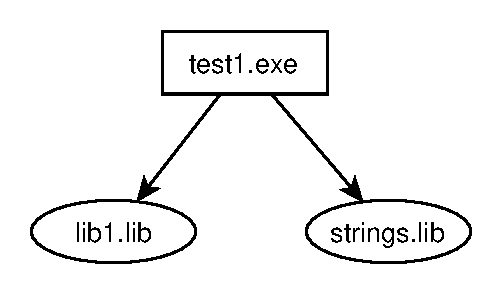
\includegraphics[width=5cm,keepaspectratio]{sample1/test1-6a.pdf}}
\end{minipage}
&&
\begin{minipage}[t]{5cm}
\center{Win32 link \vspace{0.2cm}}
\fbox{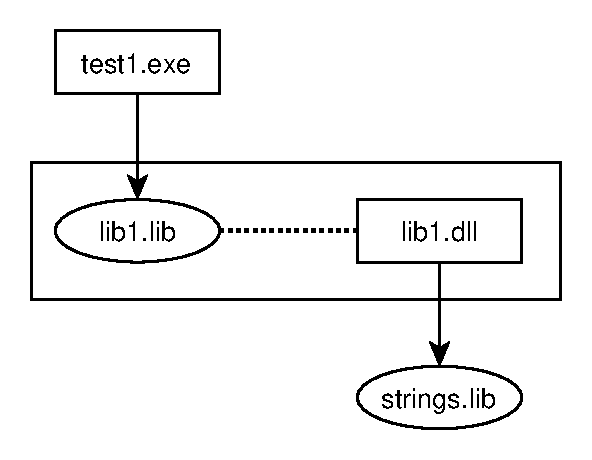
\includegraphics[width=5cm,keepaspectratio]{sample1/test1-6b.pdf}}
\end{minipage}
\end{tabular}
\end{center}
\end{figure}

\begin{figure}[h!]
\caption{\label{sample1.6:diffusion-graphs} \nameb{test1} Diffusion Graphs}
\begin{center}
\begin{tabular}[t]{ccc}
\begin{minipage}[t]{4cm}
\center{VxWorks diffusion \vspace{0.2cm}}
\fbox{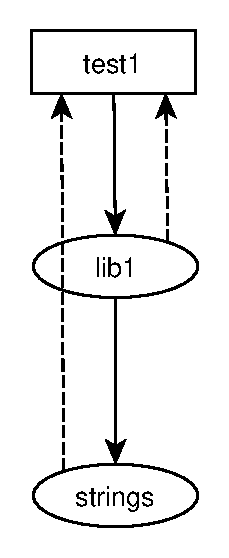
\includegraphics[height=4cm,keepaspectratio]{sample1/test1-6d.pdf}}
\end{minipage}
&&
\begin{minipage}[t]{4cm}
\center{Win32 diffusion \vspace{0.2cm}}
\fbox{\includegraphics[height=4cm,keepaspectratio]{sample1/test1-6c.pdf}}
\end{minipage}
\end{tabular}
\end{center}
\end{figure}

\clearpage

How \freemason\ handles those link scenarios in the most compact way? Through a semantics of \concept{module product diffusion}.
Examine the diffusion graphs in Figure \ref{sample1.6:diffusion-graphs}. Notice that at
the base of the diffusion graph lies a common module dependency graph, that reflects the relation between symbol definition and
usage in terms of modules (that is, if module M1 defined a symbol that is used by module M2, we say that M2 depends on M1).
\par
Now, in the module dependency graph, some modules let products of dependant modules "diffuse" through, while other do not.
The quality of diffusion is determined solely by module type. For instance, on VxWorks, a library (\nameb{lib1}) will let
another library (\nameb{strings}) diffuse into a program (\nameb{test1}), where it would be linked.
On the other hand, on Win32, a DLL (\nameb{lib1}) will not allow a library (\nameb{strings}) to diffuse through, and link it by itself.

This is the point to mention that we can request \freemason\ to print dependency graphs and
diffusion graphs. Due to the potential complexity of such graphs, \freemason\ prints them as
trees (by repeating nodes where needed).
\par
Printing a dependency graph is done with the command
\begin{center}
\fbox{\texttt{mk PLATFORM=win32 DEBUG=1 show-deps}}
\end{center}
(\verb"PLATFORM=vxworks" yields the same result)

\begin{figure}[h]
\caption{\label{sample1.6:depends-report}\nameb{test1} Dependencies and Diffusion Report}

\begin{center}
\begin{tabular}{ccccc}

\begin{minipage}[t]{4cm}
\center{Dependencies}
%\caption{\label{sample1.6:show-deps}}
\begin{Code}
test1 []
... lib1 [test1]
... ... strings [lib1]
\end{Code}
\end{minipage}

&&

\begin{minipage}[t]{5cm}
\center{Win32 Diffusion}
%\caption{\label{sample1.6:show-diffuse-win32}}
\begin{Code}
test1 []
... lib1 [test1]
... ... strings [lib1]
        >> LIB: strings.lib
    >  LIB: strings.lib
    >> SO: lib1.lib
>> SO: lib1.lib
\end{Code}
\end{minipage}

&&

\begin{minipage}[t]{5cm}
\center{VxWorks Diffusion}
%\caption{\label{sample1.6:show-diffuse-vxworks}}
\begin{Code}
test1 []
... lib1 [test1]
... ... strings [lib1]
        >> LIB: strings.a
    >  LIB: strings.a
    >> LIB: lib1.a strings.a
>> LIB: lib1.a strings.a
\end{Code}
\end{minipage}

\end{tabular}
\end{center}
\end{figure}

A few words about the reports on Figure \ref{sample1.6:depends-report}:
\begin{enumerate}
	\item Module that appears in square brackets is the parent module of the one listed to their left.
	\item Lines that begin with \verb">" list modules that are trying to diffuse through the module
		on the same level of indentation. For instance, line 5 tells us that the library \verb"strings.lib" is
		trying to diffuse through module \nameb{lib1}.
	\item Lines that begin with \verb">>" list modules that have successfully diffused through the module
		on the same level of indentation. For instance, line 6 tells us that is Win32, the link library \verb"lib1.lib"
		has diffused through module \nameb{lib1}, whereas in VxWorks, both \verb"lib1.a" and \verb"strings.a" have
		managed to do the same.
	\item The last line in the diffusion reports tells us what products will take part of the build process of the
		root module (in this case, \nameb"test1").
\end{enumerate}

\clearpage
% ---------------------------------------------------------------------------------------------
%\section{Prebuilt Modules}
%TBD: make strings prebuilt

% ---------------------------------------------------------------------------------------------
\part{Digging Deeper, Building Higher}

% ---------------------------------------------------------------------------------------------
\chapter{\freemason\ Architecture}

The \freemason\ world is composed of source code organized into \textit{modules}, each of which
containing source files to be built into a \textit{product} (mostly a binary file such as a library or an executable).
Products may be built for numerous \textit{targets} (a general name for operating systems and hardware architectures -
CPU, board, etc.) using a selection of \textit{tools} (i.e., compilers).
In order to reduce complexity of target specification, we use an arbitrary concept of \textit{platform} to
denote a particular selection of target OS, target architecture, and build tools. So, in order for \freemason\ to
get a clear notion of what is expected from it, one needs only specify the target platform.
\\
Apart from its source files, a module may require the products of other modules in order to build its own.
We denote such modules \textit{dependant modules} or just \textit{module dependencies} (not to be confused with dependencies
of C/C++ source files on header files, to which we refer as \textit{source file dependencies}).
For example, if module A uses a function f() that is defined by module B (Figure ?), we say that module A depends on module B.
If products of dependant modules are not available in advance, they should be built before they are required by their dependee.
This operation has a recursive manner, since dependant modules may have dependencies of their own.
\freemason\ allows modules to specify their dependencies and efficiently takes care of the recursive build
operation in a process called \textit{deep build}.

\begin{figure}[h]
\caption{Module dependencies}
\begin{center}\fbox{\includegraphics[width=7cm]{freemason-modules-1.jpg}}\end{center}
\end{figure}

\section{Framework}
    \freemason\ is essentially a combination of makefiles, organized in a hierarchical structure.
	This collection of makefiles is denoted \concept{Freemason Framework} or simply \concept{Framework}.
	The actual framework files that are used during a Freemason session depend on
	the session configuration (that is, values of configuration variables, such as \verb"PLATFORM" or \verb"DEBUG").
	The framework is of a dynamic nature, and may change from time to time. In the most common scenario,
	the framework is a treated part of the source code it used to compile, and therefore holds the same
	version control markers (i.e. labels) as the source code.

\section{View}
    \freemason\ assumes that the file system containing source files in a given build session share a common root directory.
    The directory structure is called \concept{view}. The common root directory is called \concept{view root}.
    The only exceptions to this rule are SDK files and the \freemason\ Framework files. It is highly recommended to keep the
    \freemason\ Framework inside the view, especially when a source control system is involved.

\section{Repository}
    In order for \freemason\ to be able to perform actual compilations, it needs to be able to access build tools (i.e. compilers)
	and SDK resources (header files and libraries). Although it is possible to configure \freemason\ to use such resources from
	the host that runs the compilation, it is sometimes easier to rely on a common, stable resources. Such resource are stored
	in a location that's called \textit{Repository}, typically in a shared network location.
	Since such resources are not always subject to version control, it should contain explicit version specification as part
	of the directory structure, and avoid modification of the standard, "off-the-self" packages of the development tools.
	\freemason\ uses the \verb"NBU_BUILD_ROOT" environment variable to locate its repository.

\section{GNU make}
    The engine that drives \freemason\ is GNU make with syntax extension.
    Thus, the definition files of \freemason\ are actually makefiles. The basic GNU make syntax is valid in \freemason\ files,
    including variable definitions, conditional control structures and 'include' directives.
    See also appendix ? for detailed description of syntax additions and changes to the standard GNU make language.

\section{Software Modules}
    A \freemason\ module is either a white-box, a black-box, or both. A black-box module is one that
    \"knows\" how to build itself from its source files. A black-box module is one that can be referenced and used by
    other modules (i.e., a module that represents a library that can be linked to an application).
    Both kind of modules may have dependant modules.
    \\
    White-box modules own a \verb"makefile" file. Black-box modules own a \verb"defs.mk" file. Module dependencies are described
    in a \verb"depends.mk" file. Those are the basic \freemason\ module description files. Modules may also have any number of arbitrary
    makefiles, that may be references (mostly, included) from the basic \freemason\ module description files.
    \\
    In a typical (and also, recommended) configuration, \freemason\ module description files reside next to the module's source files.
    However, there's no rule against putting them anywhere in the system, as long as they are kept together. In this case, we should tell
    \freemason\ how to find the module's source files.

\section{Environment Variables}
    \freemason\ intentionally tries to avoid using of environment variables, to avoid miss-configuration of the build process.
    An exception to the rule is the variable \verb"NBU_BUILD_ROOT", which points to the root of the \concept{Freemason Repository}.
	All configuration aspects should be handled from within the \freemason\ module configuration files or from the \concept{Framework}.

% ---------------------------------------------------------------------------------------------

\newpage
\watermarkgraphic{}%
\watermark%
\draftstring{Draft}%
\draftfontsize{150}%

% ---------------------------------------------------------------------------------------------
\chapter{Interaction}

\freemason\ services are provided through a single command (also called "driver"): \textbf{mk}.
All operations concerning a module are performed from the directory containing its definition files.
The driver resides at the \freemason\ Repository, and serves as a dispatcher to the GNU make utility in the
active view, so the right version is used.
\par
The parameters we supply to the driver divide into three categories:
\begin{itemize}
    \item Goals: single words, mostly in lowercase. Each goal stands for an action. While it is possible to specify
        more than one goal in a single command, it is sometimes better to limit ourselves to one goal per command, because
        different goals may have arguments (variables) with similar names. It is also possible not to specify a goal at all.
        In this case, the default goal is taken: \freemason\ builds the project.
    \item Variables: terms of the form VARIABLE=value. Some variables have a general meaning, while others are relate to a specific goal.
    \item \verb"GNU make" command-line options. See appendix ?.
\end{itemize}
The parameters may appear in any order.

% ---------------------------------------------------------------------------------------------
\section{Some basic examples}

There is one thing \freemason\ has to know before it can build a project: what is the platform for which we want to build. Therefore,
we should set the variable \verb"PLATFORM" to one of the following:
\begin{itemize}
    \item \verb"rv-win32"
    \item \verb"rv-755"
    \item \verb"rv-tamar"
\end{itemize}
As said earlier, there is nothing special about those platforms. They are just a combination of configuration settings. Those names aren't
hard-coded anywhere. For instance, if we define a new platform with the same attributes as one of the platforms listed above and build it,
the results will be exactly the same as if we used the original one.
\\
For C/C++ projects, another setting is required: whether we require debug information (\verb"DEBUG=1") or we prefer
an optimized build (\verb"OPT=1"). Those settings are mutually exclusive.

% ---------------------------------------------------------------------------------------------
\chapter{Modules}

A module owns three definition files, describing its properties:
\begin{itemize}
  \item{\verb"makefile"}
  \item{\verb"defs.mk"}
  \item{\verb"depends.mk"}
\end{itemize}

%TBD: deep build
%TBD: prebuilt products

% ---------------------------------------------------------------------------------------------
\chapter{Configuration}

% ---------------------------------------------------------------------------------------------

\section{Product}
Supported products include:
\begin{description}
  \item[prog] Windows executable or VxWorks .out/.fls file
  \item[lib] Library (archive)
  \item[so] Shared Object (DLL) (Windows only)
  \item[pl] Partially-linked Object (VxWorks only)
  \item[winapp] Windows Application
  \item[mfcapp] Windows MFC Application
  \item[none] No product (used in products that do nothing but probably get paid quite a lot)
\end{description}

% ---------------------------------------------------------------------------------------------
\section{Target OS}
Supported target operating systems include (via \verb"$(TARGET_OS)"):
\begin{description}
  \item[win32] Windows
  \item[vxworks-5.5] VxWorks 5.5
  \item[vxworks-6.3] VxWorks 6.3
\end{description}
Target OS types (via \verb"$(TARGET_OS_TYPE)"):
\begin{description}
  \item[windows] Windows
  \item[vxworks] VxWorks
\end{description}

% ---------------------------------------------------------------------------------------------
\section{Target Platform}
Currently defined target platforms:
\begin{description}
    \item[rv-win32]Windows platform
        \begin{description}
            \item[Target OS]Windows
            \item[Target Architecture]x86
            \item[CC tool] Microsoft C/C++ Compiler version 12.0
        \end{description}
    \item[rv-755]RV755 platform
        \begin{description}
            \item[Target OS] VxWorks 5.5
            \item[Target Architecture] RV755 board
            \item[CC tool] Diab 5.0
        \end{description}
    \item[rv-tamar]TAMAR platform
        \begin{description}
            \item[Target OS] VxWorks 6.3
            \item[Target Architecture] TAMAR board
            \item[CC tool] Diab 5.4
        \end{description}
\end{description}

% ---------------------------------------------------------------------------------------------
\chapter{Builder Host}

\freemason\ does not require installation of any development tool, IDE or SDK. However, if one wishes
that \freemason\ will use such a component, it is easy to establish such configuration without modifying
the framework.

% ---------------------------------------------------------------------------------------------
\chapter{Goals}

% ---------------------------------------------------------------------------------------------
\chapter{The Repository}
%TBD when traveling.

% ---------------------------------------------------------------------------------------------
\chapter{Modules Revisited}

% ---------------------------------------------------------------------------------------------
\section{Source Files}

% ---------------------------------------------------------------------------------------------
\section{Writing Module Definitions Files}

% ---------------------------------------------------------------------------------------------
\section{Source file dependencies}

% ---------------------------------------------------------------------------------------------
\section{Module dependencies}

% ---------------------------------------------------------------------------------------------
\section{Writing Module-Dependency Files}

% ---------------------------------------------------------------------------------------------
\chapter{C/C++ Preprocessing Facilities}

% ---------------------------------------------------------------------------------------------
\chapter{Reference}

% ---------------------------------------------------------------------------------------------
\section{Make Targets}
\begin{description}
  \item[cc]
  \item[cpp]
  \item[clean]
  \item[install]
  \item[show-deps]
\end{description}

% ---------------------------------------------------------------------------------------------
\section{Installation}

\begin{enumerate}
\item Define the \verb"NBU_BUILD_ROOT" environment variable to \verb"r:/build" (we assume \verb"r:" is mapped to \verb"\\storage\\NBU\\Build").
\item Append the directory \verb"%NBU_BUILD_ROOT%\sys\scripts\bin" to the back of your PATH.
\end{enumerate}

\freemason\ does not require installation of any development tool, IDE or SDK. It is planned to coexist with development
tools installed locally on a builder host. It can, however, use the resources on that host if requested. More on that
later.

% ---------------------------------------------------------------------------------------------
\section{Variables}
\begin{description}
  \item[DEEP]
  \item[SHOW\_CMD]
  \item[SHOW\_DEPS]
  \item[SHOW\_DIFFUSE]
  \item[FILE]
\end{description}

% ---------------------------------------------------------------------------------------------
\subsection{Useful MAKE options}
\begin{description}
  \item[-n]
  \item[-jN]
  \item[-k]
  \item[-B]
  \item[-P]
  \item[-v]
\end{description}

% ---------------------------------------------------------------------------------------------
\section{Target Architectures}
Currently, the concept of target architecture corresponds to the target system's CPU.
\paragraph{Supported target architectures include:}
\begin{description}
  \item[x86] Standard Intel-based PC
  \item[ppc-604] RV755 board
  \item[ppc-85xx] TAMAR board
\end{description}

% ---------------------------------------------------------------------------------------------
\section{Build Tools}
\paragraph{Supported build tools include:}
\begin{description}
  \item[msc-12] Microsoft C/C++ Compiler version 12.0 (i.e. Visual Studio 6)
  \item[diab-5.0] Diab 5.0 (i.e. VxWorks 5.5, Tornado 2.2)
  \item[diab-5.4] Diab 5.4 (i.e. VxWorks 6.3, Workbench 2.5)
  \item[diab-5.5] Diab 5.5 (i.e. VxWorks 6.3, Workbench 2.6)
  \item[cc] CC (C/C++ compiler abstraction)
  \item[asn.1] ASN.1 compiler
\end{description}

\paragraph{Additional tools we plan to support:}
\begin{itemize}
  \item GCC C/C++ Compiler
  \item Flex and Bison
\end{itemize}

% ---------------------------------------------------------------------------------------------
\section{Other development tools}
Those tools are not categorized as primary build tools, but may take part in the build process
or provide useful information during development. They are accessible through specification of a
\textsl{MAKE target} or a MAKE variable.
\paragraph{Supported tools:}
\begin{itemize}
  \item GNU CPP (C preprocessor)
\end{itemize}

\paragraph{Additional tools we plan to support:}
\begin{itemize}
  \item PC-Lint
  \item BoundsChecker, Insure++ (memory debugging tools for Windows)
  \item BullseyeCoverage (coverage analysis tool)
  \item ElectricFence, Valgrind (memory debugging tools for Linux)
\end{itemize}

% ----------------------------------------------------------------
\end{document}
% ----------------------------------------------------------------
